\documentclass[12pt,a4paper]{report}
\usepackage[utf8]{inputenc}
\usepackage[spanish]{babel}
\usepackage{amsmath}
\usepackage{amsfonts}
\usepackage{amssymb}
\usepackage{makeidx}
\usepackage{graphicx}
\usepackage[left=1cm,top=1cm,right=1cm,bottom=1cm]{geometry} 
\title{Desarrollo}
\usepackage{float}
\begin{document}
	\begin{center}
		\begin{Large}
			Desarrollo.\\
			\vspace{1.5cm}
		\end{Large}
	\end{center}
\begin{flushleft}
	Lo primero que hicimos fue obtener los valores de cada una de las resitencias y compararlo con el  valor obtenido en la medici\'on, para ello nos apoyamos en una tabla del codigo de colores como la que se muestra a continuaci\'on:\\
	\vspace{0.5cm}
\begin{figure}[H]
	\centering
	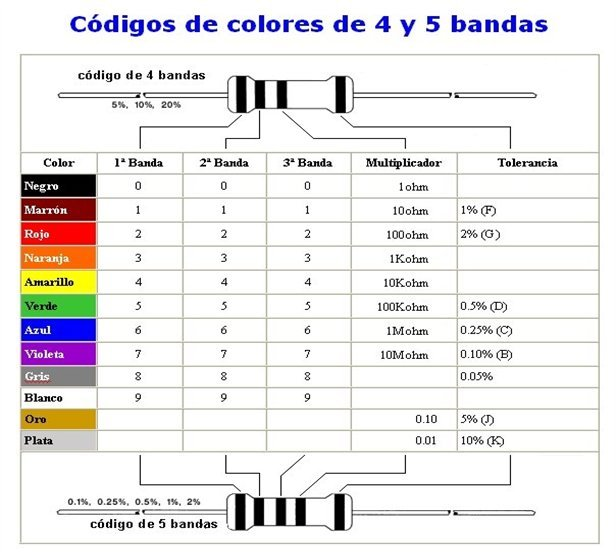
\includegraphics[width=0.4\linewidth]{bandas}
	\label{fig:bandas}
	\vspace{0.5cm}
\end{figure}
	
	\begin{large}
		Resistencia 1.\\
	\end{large}

	La primer muestra de resistencia que medimos tenia un c\'odigo de colores de rojo, rojo, rojo, dorado como se muestra en la figura.\\
	\begin{figure}[H]
		\centering
		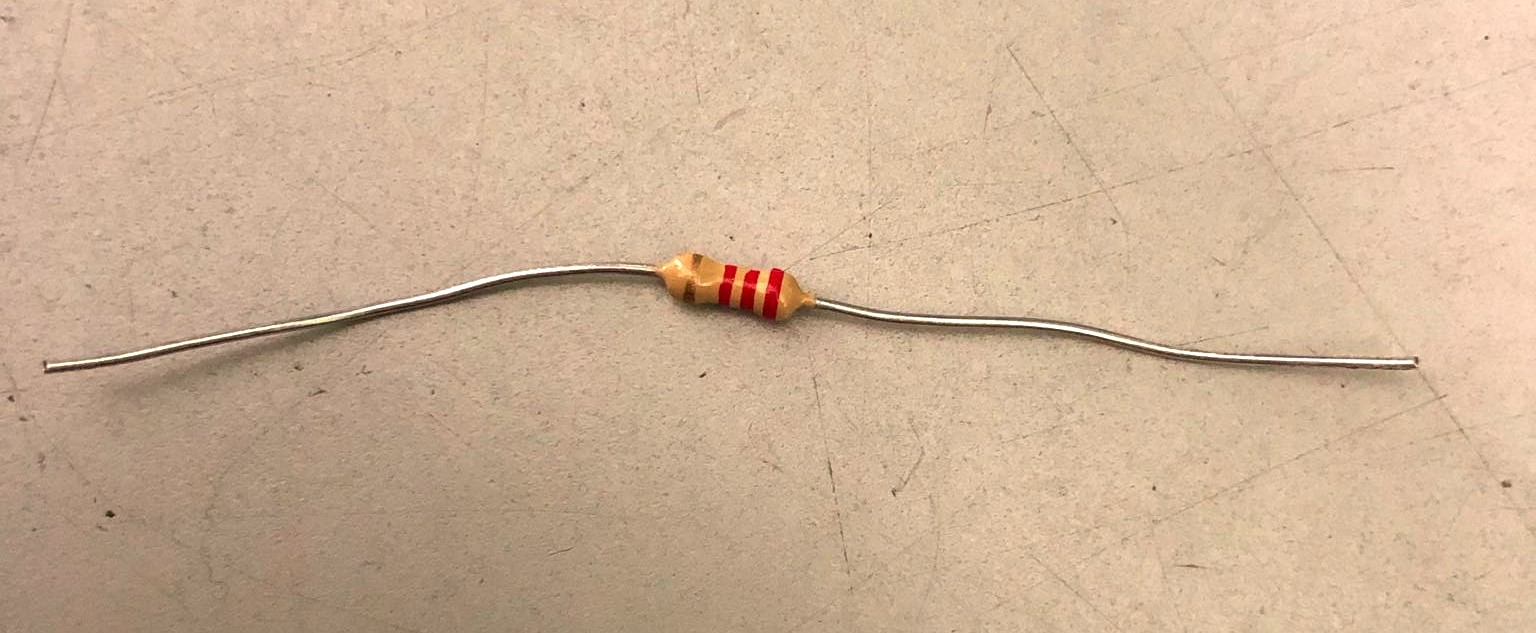
\includegraphics[width=0.4\linewidth]{resistencia1}
		\label{fig:resistencia1}
	\end{figure}

	Por lo tanto el valor de la resistencia es de 2200 ohms o 2.2 kohms.\\
	Y la medici\'on obtenida fue de 2.19 kohms como muestra la imagen.
\begin{figure}[H]
	\centering
	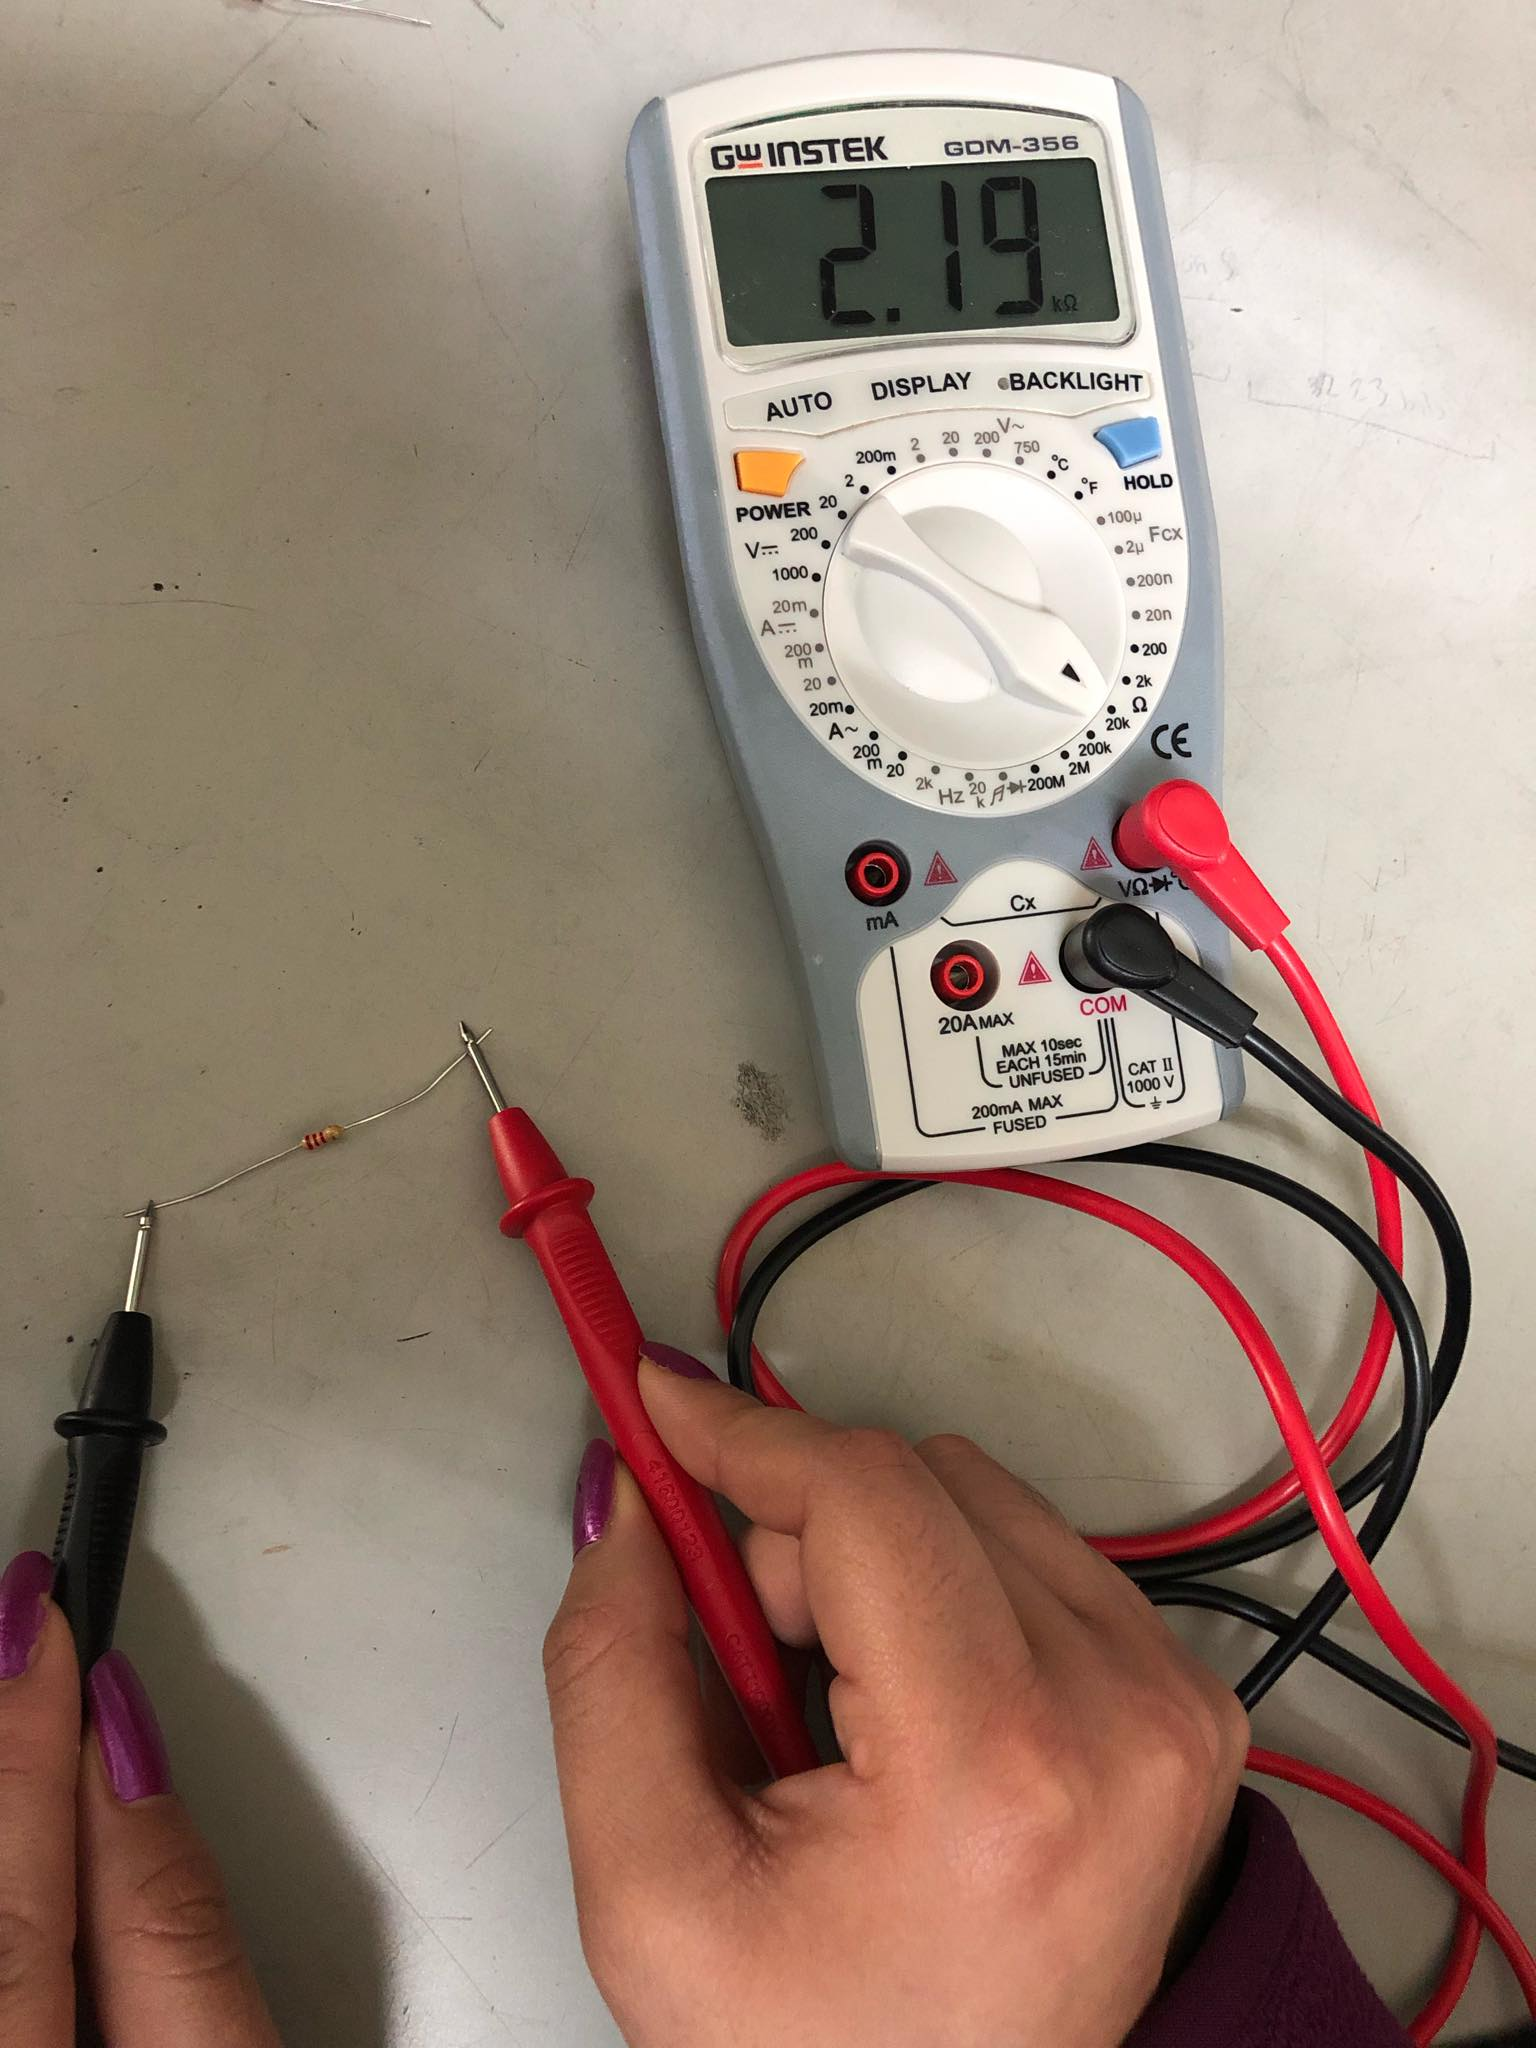
\includegraphics[width=0.3\linewidth]{medicion1}
	\label{fig:medicion1}
\end{figure}
	\clearpage

	\begin{large}
		\vspace*{2cm}
		Resistencia 2.\\
	\end{large}
	La segunda resistencia que medimos tenia un c\'odigo de colores de rojo, negro, verde y dorado, como se muestra en la imagen.\\
	
\begin{figure}[H]
	\centering
	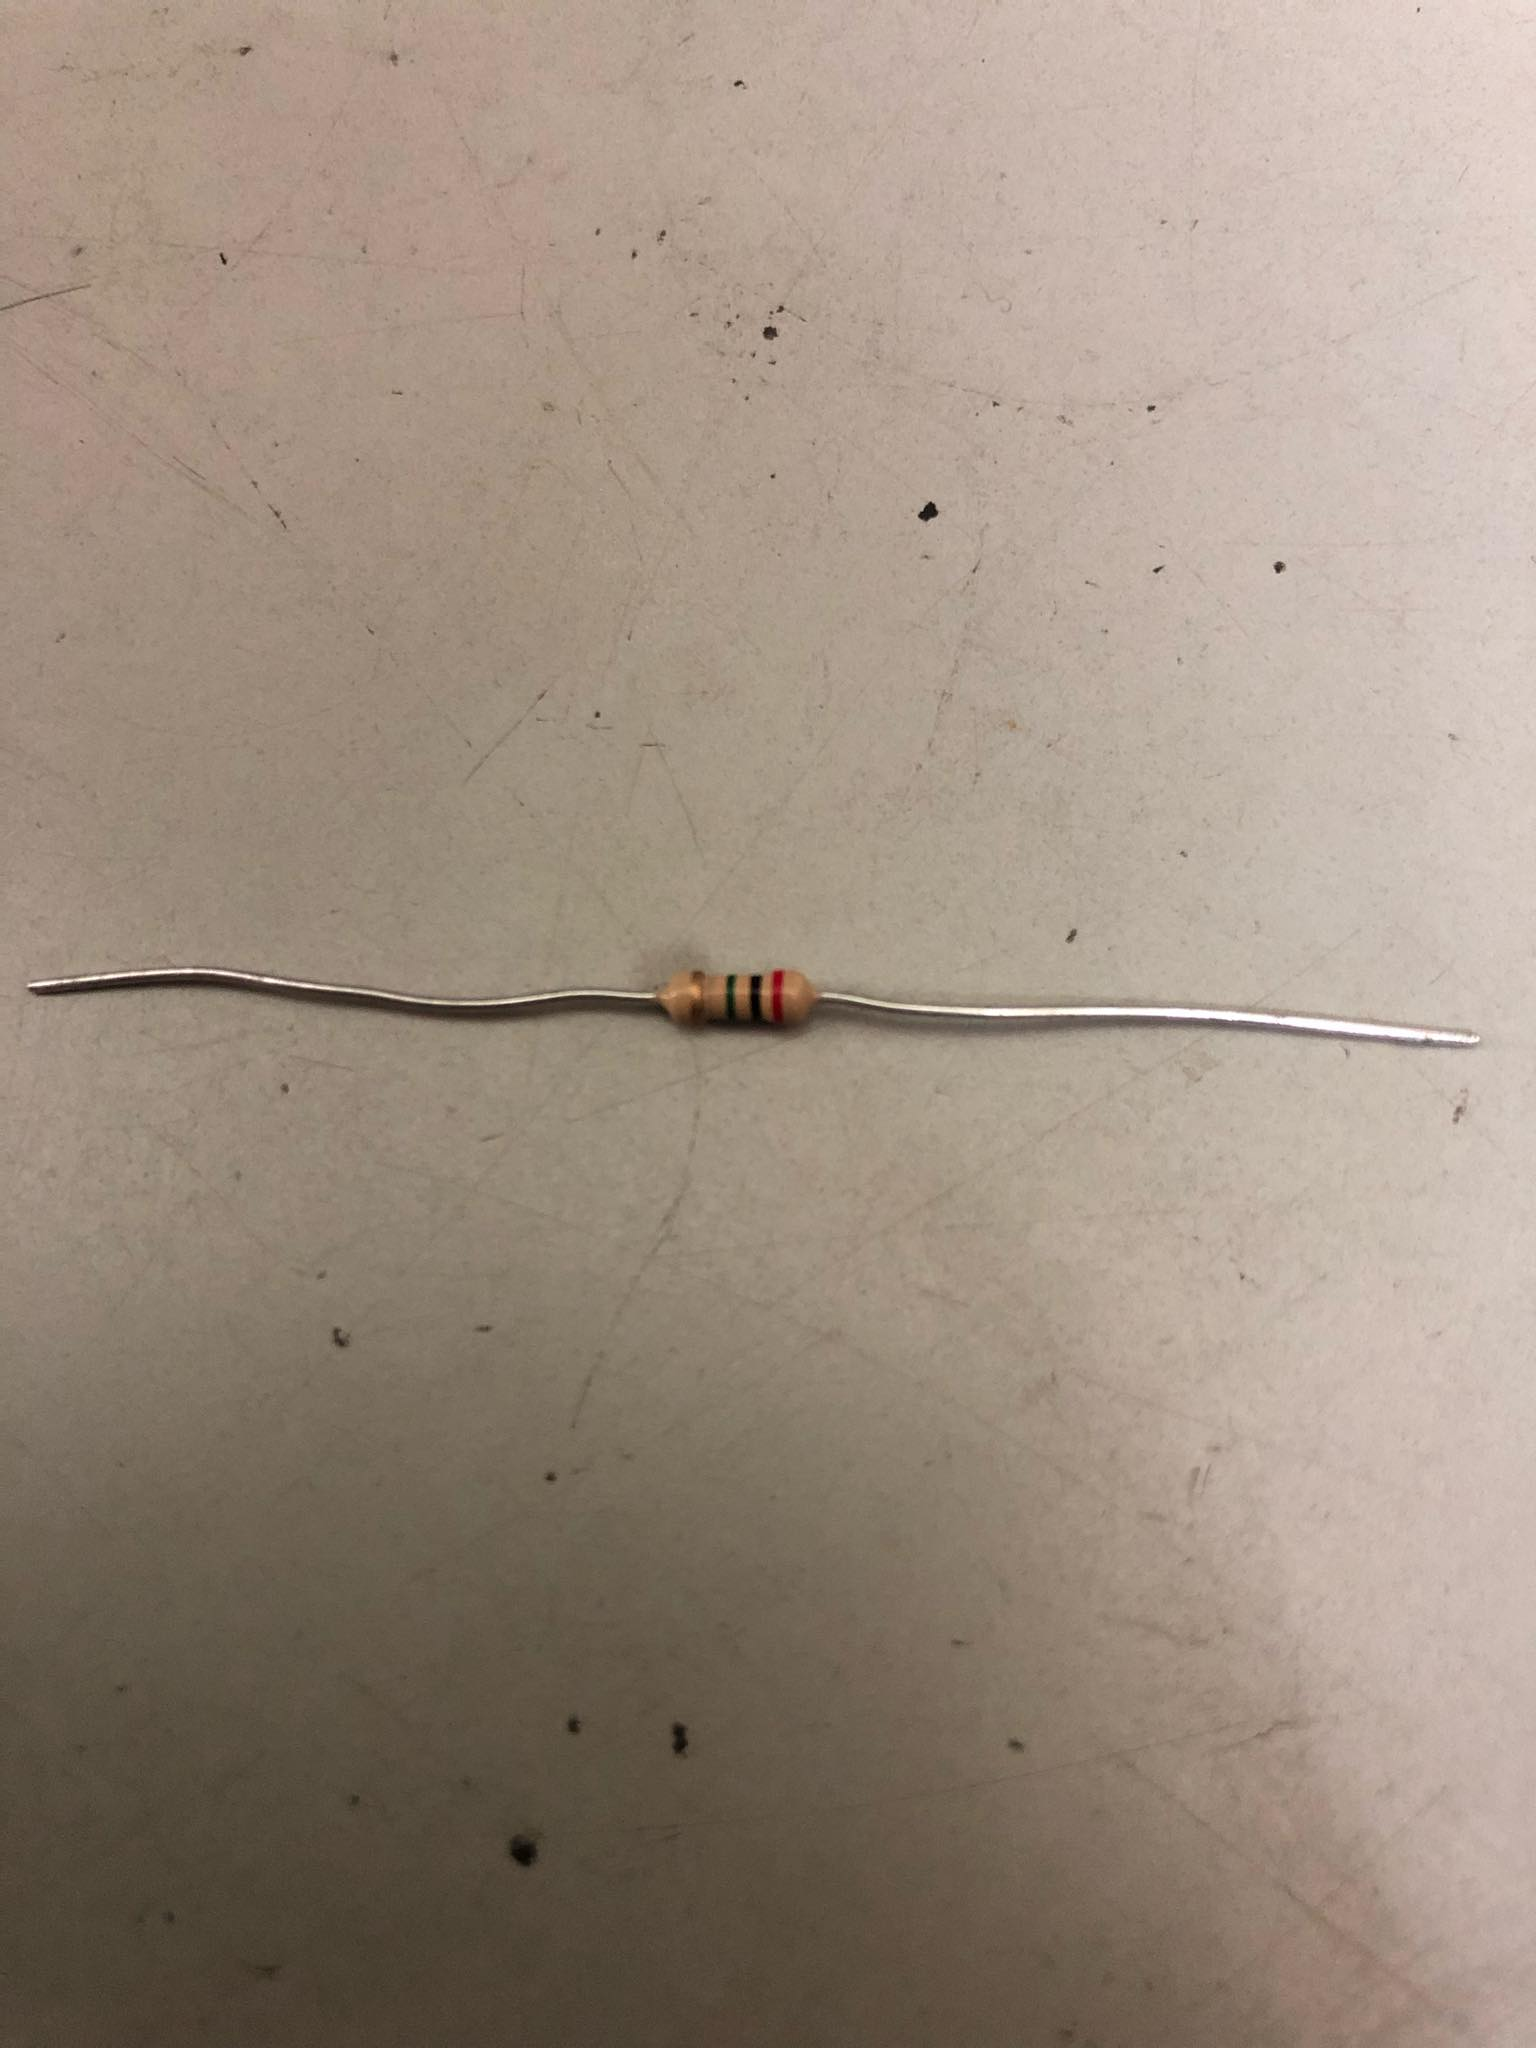
\includegraphics[width=0.4\linewidth]{resistencia2}
	\label{fig:resistencia2}
\end{figure}
 	Por lo tanto tenemos una resistencia con un valor de 2 MegaOhms.\\
 	Y la medici\'on obtenida fue de 3 Megaohms, como muestra la imagen.\\
 	\begin{figure}[H]
 		\centering
 		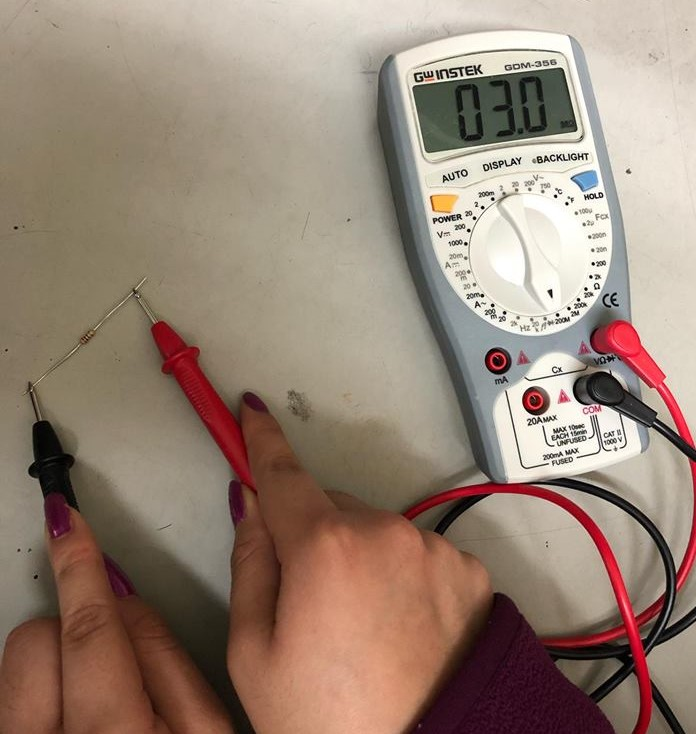
\includegraphics[width=0.3\linewidth]{medicion2}
 		\label{fig:medicion2}
 	\end{figure}
 	
 		\begin{large}
 		\vspace*{2cm}
 		Resistencia 3.\\
 	\end{large}
 	La tercera resistencia que medimos tenia un c\'odigo de colores de gris, rojo, caf\'e, y dorado, como se muestra en la imagen.\\
 	
 	\begin{figure}[H]
 		\centering
 		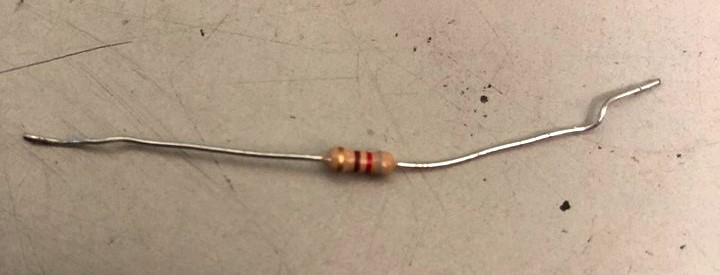
\includegraphics[width=0.4\linewidth]{resistencia3}
 		\label{fig:resistencia3}
 	\end{figure}
 	Por lo tanto tenemos una resistencia con un valor de 821 Ohms \\
 	Y la medici\'on obtenida fue de 810 Ohms, como muestra la imagen.\\
 	\begin{figure}[H]
 		\centering
 		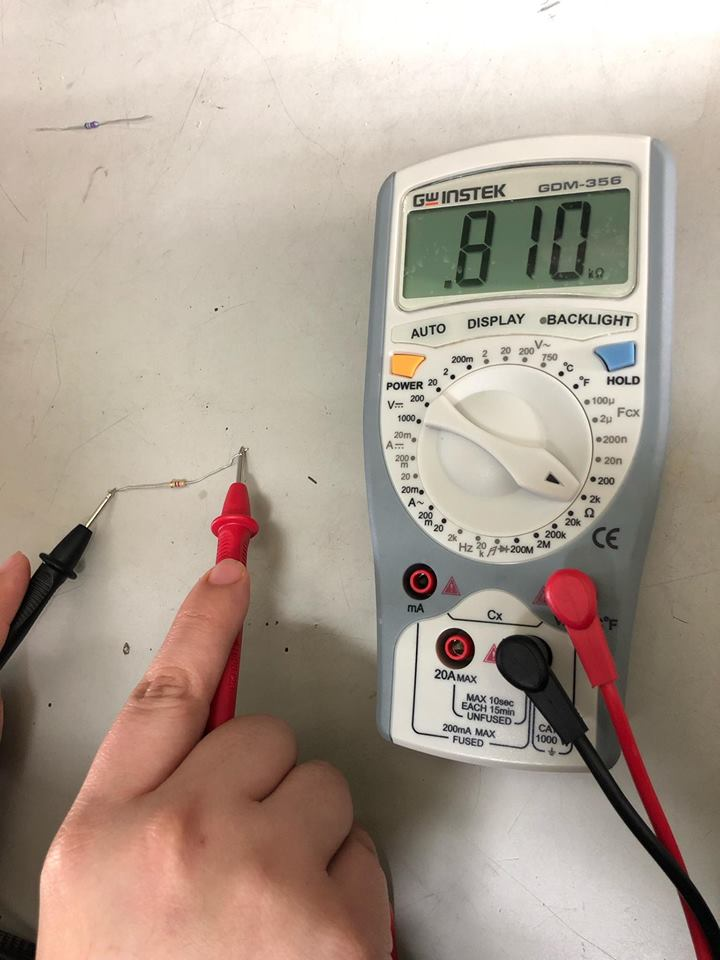
\includegraphics[width=0.3\linewidth]{medicion3}
 		\label{fig:medicion3}
 	\end{figure}
 
 	\begin{large}
 	\vspace*{2cm}
 	Resistencia 4.\\
 \end{large}
 La cuarta resistencia que medimos ten\'ia un c\'odigo de colores verde, azul,amarillo y dorado, como se muestra en la imagen.\\
 
 \begin{figure}[H]
 	\centering
 	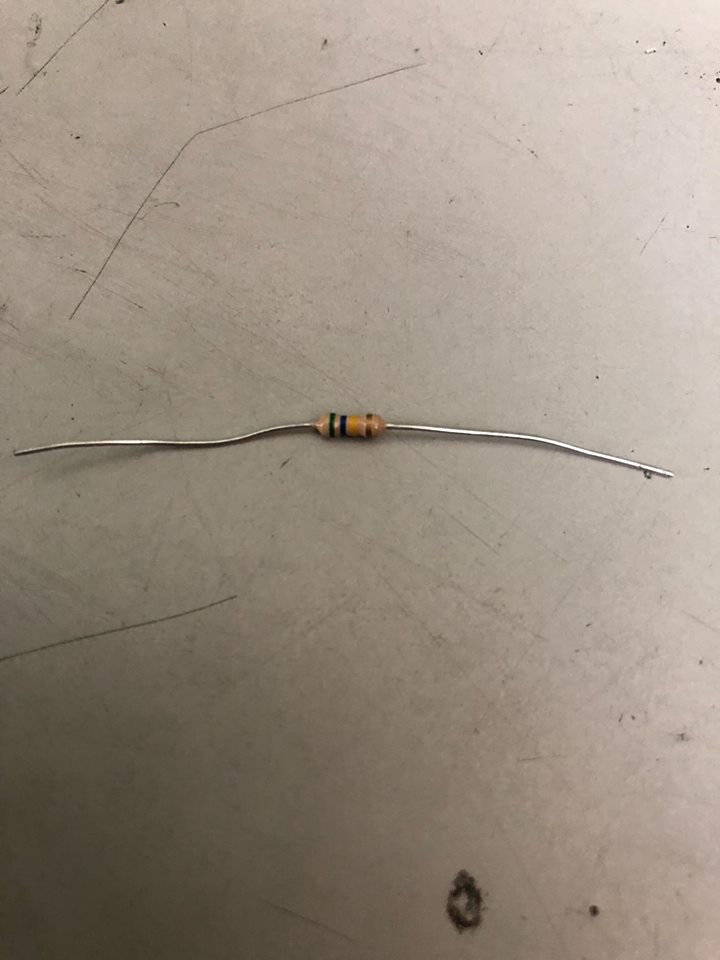
\includegraphics[width=0.4\linewidth]{resistencia4}
 	\label{fig:resistencia4}
 \end{figure}
 Por lo tanto tenemos una resistencia con un valor de 564 Ohms \\
 Y la medici\'on obtenida fue de 581 Ohms, como muestra la imagen.\\
 \begin{figure}[H]
 	\centering
 	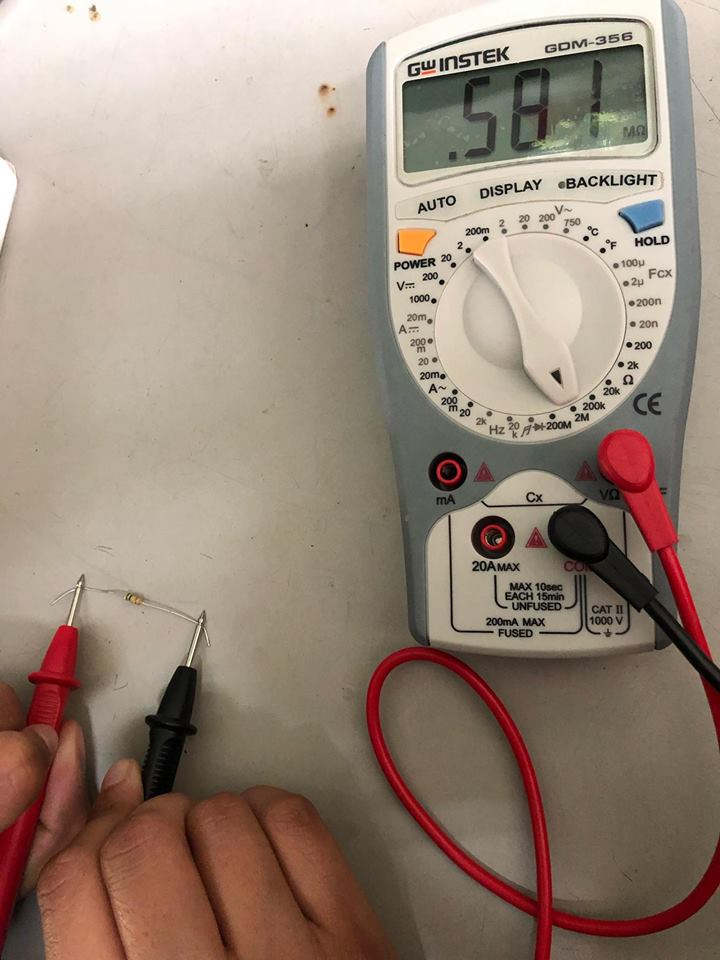
\includegraphics[width=0.3\linewidth]{medicion4}
 	\label{fig:medicion4}
 \end{figure}
	
		\begin{large}
		\vspace*{2cm}
		Resistencia 5.\\
	\end{large}
	La quinta resistencia que medimos ten\'ia un c\'odigo de colores azul, amarillo,blanco, caf\'e,y marr\'on como se muestra en la imagen.
	
	\begin{figure}[H]
		\centering
		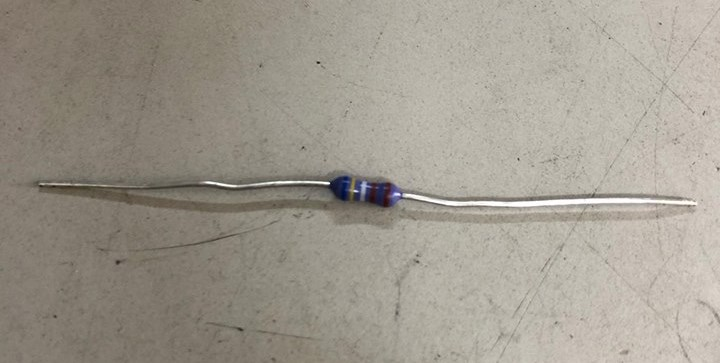
\includegraphics[width=0.4\linewidth]{resistencia5}
		\label{fig:resistencia5}
	\end{figure}
	Por lo tanto tenemos una resistencia con un valor de 6490 KiloOhms.\\
	Y la medici\'on obtenida fue de 6480 KiloOhms como se muestra en la imagen.\\
	\begin{figure}[H]
		\centering
		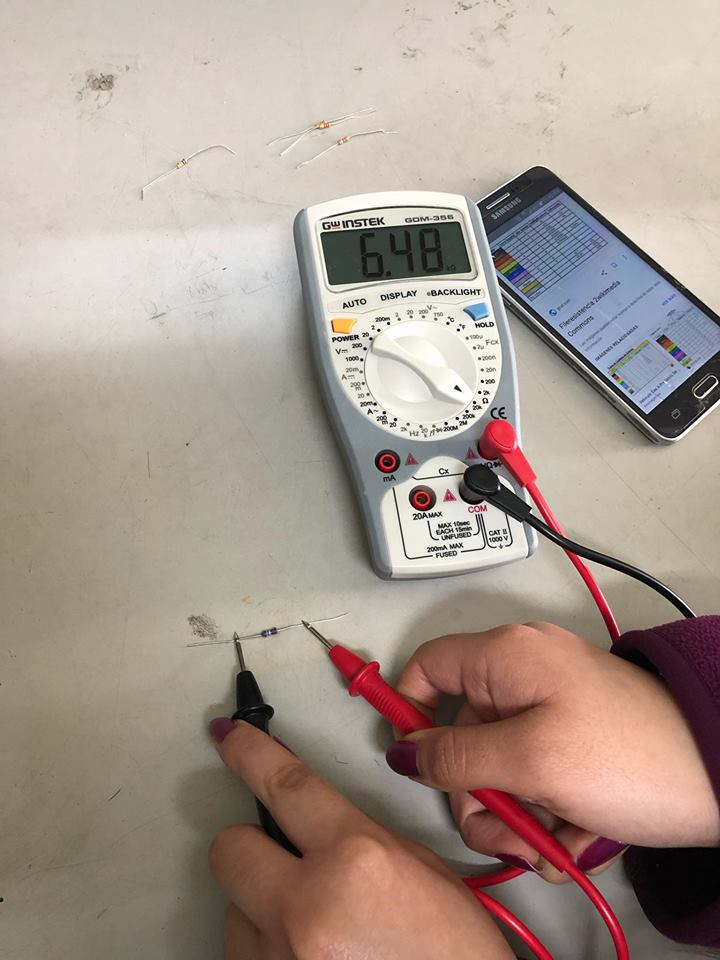
\includegraphics[width=0.3\linewidth]{medicion5}
		\label{fig:medicion5}
	\end{figure}
	
	

	 




	
\end{flushleft}
	
\end{document}